\documentclass[11pt]{article}
\usepackage{fullpage}
\usepackage{url, graphicx, amsmath}
\usepackage[english]{babel}
\begin{document}
\thispagestyle{empty}
\parindent 0pt
\vfill
\large

\begin{center}
\LARGE{\bf \textsf{CS246: Mining Massive Datasets}}\\ {\bf \textsf{Homework 4}}
\\*[4ex]
\end{center}

\section*{Answer to Question 1(a)}
\begin{table}[h]
\centering
\label{my-label}
\begin{tabular}{|l|l|l|l|}
\hline
$w$                            & $w_1$& $w_2$& $w_3$\\ \hline
Initial                        & 0    & 0    & 0    \\
After Observing Patient ID = 1 & 0    & 0    & -1/5 \\
After Observing Patient ID = 2 & 0    & 0    & -1/5 \\
After Observing Patient ID = 3 & 0    & 0    & -1/5 \\
After Observing Patient ID = 4 & 0    & -1/5 & 0    \\
After Observing Patient ID = 5 & -1/5 & -1/5 & 1/5  \\ \hline
\end{tabular}
\end{table}

\pagebreak[4]
\section*{Answer to Question 1(b)}
The Perceptron algroithm will not return a solution to those data.
Those data points are not linearly seperable.

\begin{figure}[h]
\center
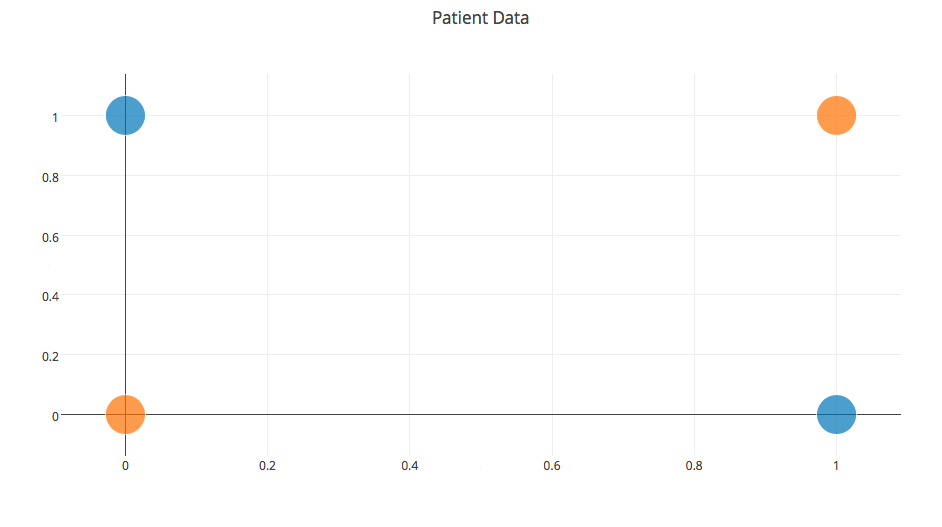
\includegraphics[scale=0.4]{patientData.png}
\caption{Patient Data}
\end{figure}

\pagebreak[4]
\section*{Answer to Question 1(c)}
From below figures it is found that only $\psi=((\phi_1 xor \phi_2),\phi_2,−1)$ is linear seperable.
The associated $w = (-1, 0, -0.5)$
\begin{figure}[h]
\center
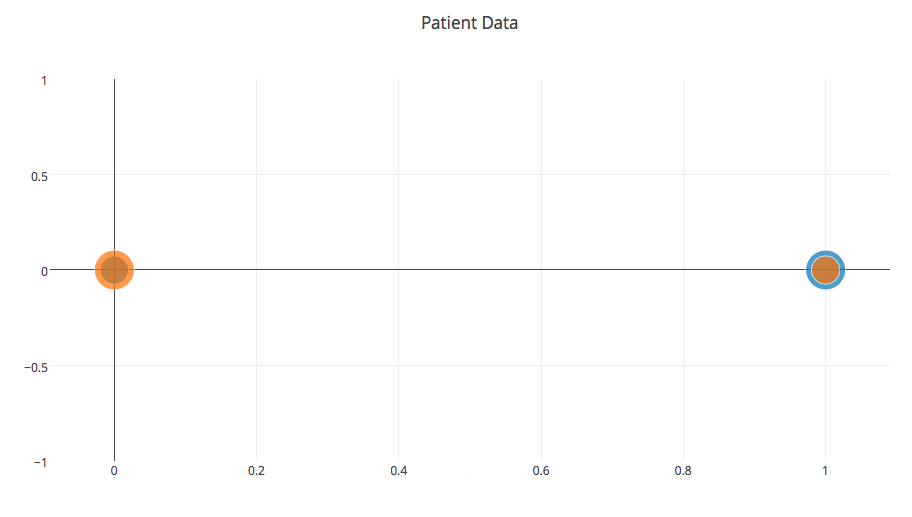
\includegraphics[scale=0.2]{patientData1.png}
\caption{$\psi = (\phi_1^2, \phi_1\phi_2, −1)$}
\end{figure}

\begin{figure}[h]
\center
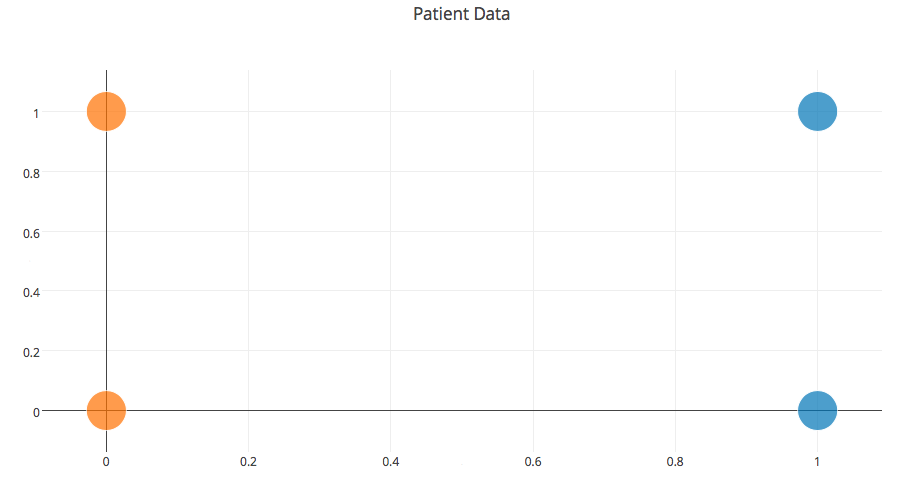
\includegraphics[scale=0.2]{patientData2.png}
\caption{$\psi=((\phi_1 xor \phi_2),\phi_2,−1)$}
\end{figure}

\begin{figure}[h]
\center
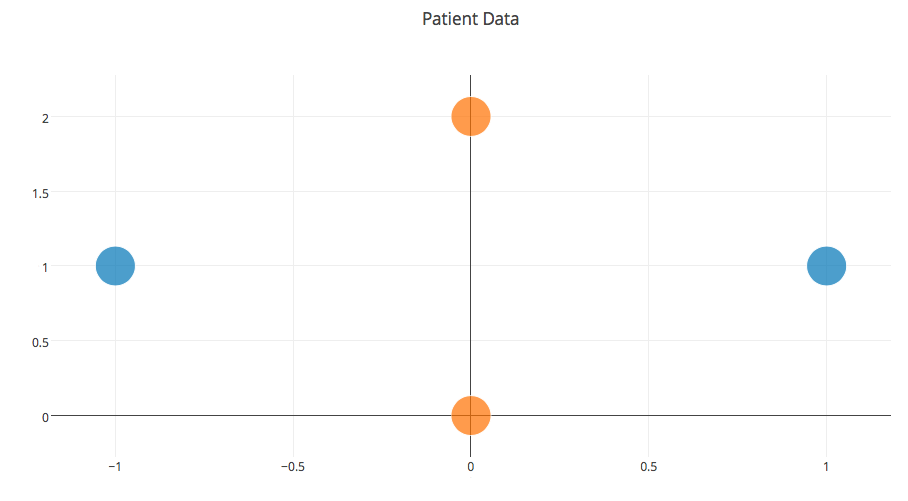
\includegraphics[scale=0.2]{patientData3.png}
\caption{$\psi=(\phi_1 - \phi_2,\phi_1 + \phi_2,−1)$}
\end{figure}

\pagebreak[4]
\section*{Answer to Question 2(a)}
$$
\nabla_b f(w, b) = C\sum_{i=n}^{n}\frac{\partial L(x_i, y_i)}{\partial b}
$$
Where:
$$
\frac{\partial L(x_i, y_i)}{\partial b} =
  \begin{cases}
    0       & \quad \text{if } y_i(x_i w + b) \geq 1\\
    -y_i  & \quad \text{if } otherwise.\\
  \end{cases}
$$

\pagebreak[4]
\section*{Answer to Question 2(b)}
From the plot below, it can be seen that stochastic gradient descent takes more iterations than the other methods.
Batch gradient descent takes less iterations. However, during each iteration for batch gradient descent,
it actually loops through the whole training set. Therefore, batch gradient descent takes more memory and it is computaion intensive.\\
\\
When comparing minibatch and SGD, minibatch takes less time than SGD even the overall computation cost for minibatch is higher.
For minibatch, it can do computation in parralel when summing over the 20 samples within the batch.
Another advantage for minibatch gradient descent is minibatch is more stable and smoother, while sometimes SGD stops running even it has not converged yet.

\begin{figure}[h]
\center
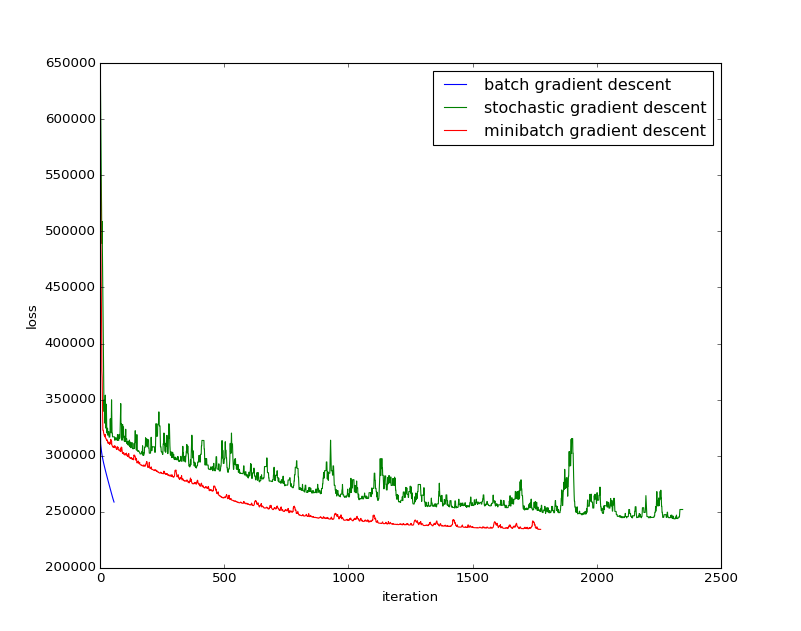
\includegraphics[scale=0.5]{gradientDescent.png}
\caption{gradient descent comparision}
\end{figure}

\pagebreak[4]
\section*{Answer to Question 3(a)}
For wine:
$$
\begin{aligned}
  G & = I(D) - (I(D_L)+I(D_R))\\
  & = 100(1-(60/100)^2-(40/100)^2) - (50(1-(3/5)^2-(2/5)^2) + 50(1-(1-(3/5)^2-(2/5)^2)))\\
  & = 48 - (24+24)\\
  & = 0
\end{aligned}
$$

For running:
$$
\begin{aligned}
  G & = I(D) - (I(D_L)+I(D_R))\\
  & = 100(1-(60/100)^2-(40/100)^2) - (30(1-(2/3)^2-(1/3)^2) + 70(1-(4/7)^2-(3/7)^2))\\
  & = 48 - (13.33 + 34.29)\\
  & = 0.38
\end{aligned}
$$

For pizza:
$$
\begin{aligned}
  G & = I(D) - (I(D_L)+I(D_R))\\
  & = 100(1-(8/10)^2-(2/10)^2) - (80(1-(5/8)^2-(3/8)^2) + 20(1-(1/2)^2-(1/2)^2))\\
  & = 48 - (37.5 + 10)
  & = 0.5
\end{aligned}
$$

We can see, splitting use PIZZA can maximize our gain on $G$.

\pagebreak[4]
\section*{Answer to Question 3(b)}
The decision tree should look at, it splits based on $a_1$ at the root.
When moving downwards, it take the next the attribute with the highest percentage rate.
As a result, this tree will have $2^{100}$ leaves.\\
\\
The decision tree should limit its split nodes. For this case, we can take $a_1$ as the only split node.
In a general setting, we can set a threshold for making new split during the training time.
If the gain in gini index is smaller than the threshold, there will be no new split based that attribute.
Also we can use post-pruning, if we have validation datasets, we can test from the leave to root whether each node is useful or not.
If the node does not improve error rate on the dev set, we can post-prune those nodes.

\pagebreak[4]
\section*{Answer to Question 4(a)}
$$
\begin{aligned}
Pr[\tilde{F}[i]\leq F[i] + \epsilon]
& = 1 - Pr[\tilde{F}[i] \geq F[i] + \epsilon]
\end{aligned}
$$
Give,
$$
\tilde{F}[i] = min_j\{c_{j,h_j(i)}\}
$$
Therefore, $c_{j,h_j(i)} \geq \tilde{F}[i]$; substitude this into the equation:
$$
\begin{aligned}
Pr[\tilde{F}[i]\leq F[i] + \epsilon]
& = 1 - Pr[\tilde{F}[i] \geq F[i] + \epsilon] \\
& \geq 1 - Pr[c_{j,h_j(i)} \geq F[i] + \epsilon, j]
\end{aligned}
$$
Since all the hash functions are independent:
$$
Pr[c_{j,h_j(i)} \geq F[i] + \epsilon, j] = \Pi_{j=0}^{\log{1/\delta}}Pr[c_{j,h_j(i)} \geq F[i] + \epsilon]
$$
Therefore,
$$
\begin{aligned}
Pr[\tilde{F}[i]\leq F[i] + \epsilon]
& \geq 1 - Pr[c_{j,h_j(i)} \geq F[i] + \epsilon, j]\\
& = 1 - \Pi_{j=0}^{\log{1/\delta}}Pr[c_{j,h_j(i)} \geq F[i] + \epsilon]\\
& = 1 - \Pi_{j=0}^{\log{1/\delta}}Pr[c_{j,h_j(i)} - F[i] \geq \epsilon]\\
& \geq 1 - \Pi_{j=0}^{\log{1/\delta}}\frac{E[c_{j,h_j(i)} - F[i]]}{\epsilon}\\
& \geq 1 - \Pi_{j=0}^{\log{1/\delta}}\frac{\frac{\epsilon}{e}(t-F[i])}{\epsilon}\\
& \geq 1 - \Pi_{j=0}^{\log{1/\delta}}\frac{1}{e}\\
& = 1 - (\frac{1}{e})^{\log{1/\delta}}\\
& = 1 - \delta
\end{aligned}
$$

\pagebreak[4]
\section*{Answer to Question 4(b)}
Roughly when word frequence is larger than $2 \times 10^{-5}$, the relative error is smaller than 1.
\begin{figure}[h]
\center
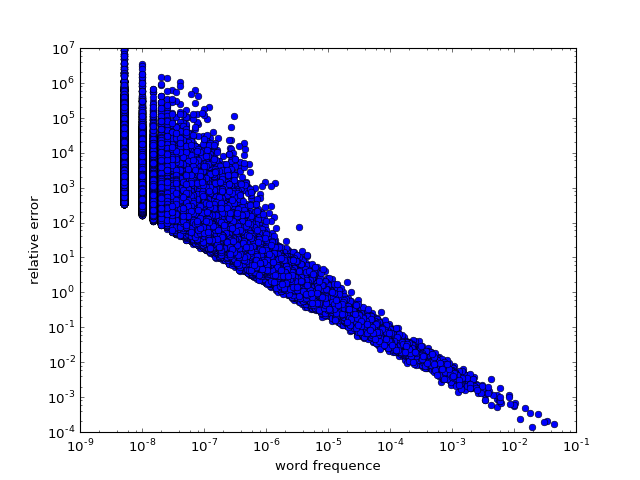
\includegraphics[scale=0.5]{streaming.png}
\end{figure}

\pagebreak[4]
\begin{center}
\LARGE{\bf \textsf{Cover Sheet}} \\*[4ex]
\end{center}

\textbf{Assignment Submission } Fill in and include this cover sheet with each of your assignments. Assignments are due at 11:59pm. All students (SCPD and non-SCPD) must submit their homeworks via GradeScope (\url{http://www.gradescope.com}). Students can typeset or scan their homeworks. Make sure that you answer each question on a separate page. Students also need to upload their code at \url{http://snap.stanford.edu/submit}. Put all the code for a single question into a single file and upload it. Please do not put any code in your GradeScope submissions.
\\
\\
\textbf{Late Day Policy } Each student will have a total of {\em two} free late periods. {\em One late period expires at the start of each class.} (Homeworks are usually due on Thursdays, which means the first late periods expires on the following Tuesday.) Once these late periods are exhausted, any assignments turned in late will be penalized 50\% per late period. However, no assignment will be accepted more than {\em one} late period after its due date.
\\
\\
\textbf{Honor Code } We strongly encourage students to form study groups. Students may discuss and work on homework problems in groups. However, each student must write down their solutions independently i.e., each student must understand the solution well enough in order to reconstruct it by him/herself.  Students should clearly mention the names of all the other students who were part of their discussion group. Using code or solutions obtained from the web (github/google/previous year solutions etc.) is considered an honor code violation. We check all the submissions for plagiarism. We take the honor code very seriously and expect students to do the same.

\vfill
\vfill

{\Large
\textbf{Your name:} \hrulefill \\
\textbf{Email:} \underline{\hspace*{7cm}} \textbf{SUID:} \hrulefill\\*[2ex] }
Discussion Group (People with whom you discussed ideas used in your answers): \\\\\\
On-line or hardcopy documents used as part of your answers: \\\\\\
\vfill

\vfill

I acknowledge and accept the Honor Code.\\*[3ex]
\bigskip
\textit{(Signed)}\hrulefill
% If you are not printing this document out, just type your initials above

\vfill
\vfill

\end{document}

